\documentclass[conf]{new-aiaa}
%\documentclass[journal]{new-aiaa} for journal papers
\usepackage[utf8]{inputenc}

\usepackage{graphicx}
\usepackage{amsmath}
\usepackage[version=4]{mhchem}
\usepackage{siunitx}
\usepackage{subcaption}
\usepackage{longtable,tabularx}
\setlength\LTleft{0pt}

% \title{Open-Vocabulary Obstruction Detection for UAS Landing via Fine-Tuned YOLO-World}
\title{Obstruction Detection for UAS Landing: Fine-Tuning YOLO-World Without Losing the Open Vocabulary}

\author{Andre Arante\footnote{Undergraduate Research Assistant, Department of Electrical and Computer Engineering, George Washington University, AIAA Student Member.}, Mahyar Ghazanfari\footnote{Ph.D. Student, Department of Mechanical and Aerospace Engineering, George Washington University, AIAA Student Member.}, Can Vu\footnote{Ph.D. Student, Department of Mechanical and Aerospace Engineering, George Washington University, AIAA Student Member.}, and Peng Wei\footnote{Associate Professor, Department of Mechanical and Aerospace Engineering, George Washington University, AIAA Associate Fellow.
}}
\affil{George Washington University, Washington, DC, 20052}

\begin{document}

\maketitle

% Abstract
\begin{abstract}

Safe autonomous landing remains a critical challenge for unmanned aerial systems (UAS)
performing package delivery, where undetected landing zone obstructions pose significant
dangers. Closed-set object detectors cannot recognize obstacles outside their training
categories, while open-vocabulary detectors such as YOLO-World can, but must be adapted to
top-down aerial imagery. This paper characterizes the tradeoff between aerial accuracy and
open-vocabulary retention when fine-tuning YOLO-World on the VisDrone dataset with its CLIP
text encoder frozen. We show that standard fine-tuning significantly degrades detection of
unseen categories within 5 epochs and turns the model into an effectively closed-set
detector by 40 epochs, and that this loss is heavily influenced by the learning rate rather than the
training duration or layer freezing. Combining a low learning rate with weight-space
ensembling (WiSE-FT) yields a model that improves VisDrone mAP@0.5 by 137\% over the
pretrained model while retaining 77--78\% of its zero-shot accuracy on LVIS and COCO and
slightly exceeding it on novel UAS obstruction categories. In an image-level landing-pad
obstruction test, this model matches the pretrained model's discrimination (AUROC 0.86)
with a 3.6$\times$ lower false-alarm rate. TensorRT FP16 inference runs at 56 FPS at
1280$\times$1280 on an NVIDIA Jetson AGX Thor with no accuracy loss, alongside real-time
results on Jetson Xavier and Orin Nano.

\end{abstract}

\section{Introduction}

The rapid expansion of unmanned aerial system
(UAS) operations in commercial logistics has positioned
autonomous package delivery as a near-term reality for
last-mile supply chains. Major operators such as
Zipline~\cite{zipline2025} and Wing~\cite{wing2025} have
already received FAA approval for beyond-visual-line-of-sight
(BVLOS) commercial operations, while companies including
Amazon, DHL, and FedEx continue to develop UAS logistics
at scale~\cite{marquand2023faa, zieher2024drones}. Despite
this momentum, safe autonomous landing remains one of the
most operationally significant unsolved challenges in the
field. The landing phase requires the UAS to localize the
landing zone and verify it is clear of obstructions, a
task made particularly difficult in dynamic last-mile
environments such as residential driveways and front yards,
where hazards range from stationary obstacles such as
vehicles and debris to dynamic ones such as pedestrians
and pets~\cite{alam2023survey}.

Previous landing systems rely on traditional closed-set object detectors such as YOLOv8~\cite{ultralytics2023} to recognize the marker from drone-mounted cameras~\cite{fattahi2017automatic, xu2024small}. While effective for marker localization, these detectors cannot generalize beyond their training categories, making them fundamentally insufficient for safe autonomous landing.

Open-vocabulary object detection (OVOD) offers a promising alternative. YOLO-World integrates a CLIP-based text encoder into the real-time YOLO framework, enabling detection of arbitrary object categories specified through natural language prompts at inference time~\cite{cheng2024yoloworld, radford2021learning}. However, deploying YOLO-World on UAS hardware requires fine-tuning on aerial datasets to close the domain gap between ground-level pretraining data and top-down drone imagery. It has been observed that fine-tuning the CLIP encoder on domain-specific data leads to severe degradation of open-vocabulary generalization, the very capability that motivates its use~\cite{cheng2024yoloworld}. Navigating this tradeoff is the central challenge this paper addresses.

This paper makes the following contributions. First, we characterize how fine-tuning
YOLO-World on the VisDrone aerial dataset, with the CLIP text encoder frozen, trades domain
accuracy for open-vocabulary retention, using controlled experiments over training duration,
learning rate, and layer freezing, evaluated on a custom UAS Open-Vocabulary Benchmark (OVB)
and on the standard LVIS, COCO, and ODinW benchmarks. We find that the learning rate, more
than the number of epochs, primarily governs forgetting. Second, we show that a low learning
rate combined with weight-space ensembling (WiSE-FT) recovers, and on novel UAS categories
slightly exceeds, the pretrained model's open-vocabulary accuracy at more than twice its
VisDrone accuracy. Third, we evaluate whether descriptive noun-phrase prompts such as
``foreign object on orange circle landing pad'' can flag obstructions that are not explicitly
prompted, at both the object level and as an image-level landing decision. Fourth, we
benchmark real-time inference on NVIDIA Jetson Xavier, Orin Nano, and AGX Thor, including
TensorRT deployment.


\section{Related Works}

\subsection{Traditional Object Detection}

One approach to the problem of autonomous UAS landing has been
through marker-based detection systems in which an ArUco marker
is placed at the landing site and detected by an onboard camera
during descent. These markers encode a unique binary pattern
that can be detected and decoded in real time using classical
computer vision techniques, allowing the UAS to estimate its
position and orientation relative to the landing zone with high
precision (Fig.~\ref{fig:aruco})~\cite{fattahi2017automatic}.
However, marker-based approaches carry one significant
limitation: they require consumers to correctly place the
marker at a landing site in advance.

In contrast, approaches have been proposed to address this
limitation. The Obstacle and Landing Site Awareness System
(OLSAS)~\cite{xu2024small} demonstrated the feasibility
of detecting a generic landing pad (Fig.~\ref{fig:landingpad}) from drone-mounted cameras without relying on ArUco markers, supporting
safe autonomous package delivery landings. These approaches
demonstrate that deep learning based landing site detection
is viable, but struggle with the fundamental limitation of
traditional closed-set detection methods: the models are
trained on a fixed list of object categories and cannot
generalize to novel obstructions not present in the training
data.


\begin{figure}[hbt!]
\centering
\begin{subfigure}{0.45\textwidth}
    \centering
    \includegraphics[height=4cm, keepaspectratio]{aruco_landing_pad.png}
    \caption{ArUco marker used in prior landing systems.}
    \label{fig:aruco}
\end{subfigure}
\hfill
\begin{subfigure}{0.45\textwidth}
    \centering
    \includegraphics[height=4cm, keepaspectratio]{general_landing_pad.jpg}
    \caption{Generic landing pad used in this work.}
    \label{fig:landingpad}
\end{subfigure}
\caption{Comparison of marker-based and marker-less landing zone
         identification approaches.}
\label{fig:landingcomparison}
\end{figure}

\subsection{Previous Approaches to Obstacle Detection for UAS Landing}

Previous work has attempted to tackle this issue of general obstacle detection in a couple different ways. A benchmarking study of closed-set detectors for small UAS autonomous landing~\cite{vu2025transformer} explored the tradeoff between convolutional neural networks (CNN) YOLOv8 and Real-Time Detection Transformer (RT-DETR). The study found that transformer based models such as RT-DETR are better suited for applications where it is necessary to optimize for uncertainty quantification to increase safe UAS landings, while CNNs like YOLOv8 are better for raw inference speed and real-time performance. However, both approaches remain constrained by the fundamental limitation of closed-set detection: neither can identify obstacles outside their fixed training categories.

To address this, the See\&Say~\cite{ghazanfari2026seesay} framework applied cloud-based vision-language models to identify safe vs unsafe landing zones and even propose alternative landing zones should the landing pad be occupied. While See\&Say offers very promising results, it is not explicitly designed for real-time operation due to latency from VLM inference and external API communication. In practice, this model could be run periodically (e.g., every 15 seconds) in order to obtain a general understanding of the environment but would require a lighter but faster model to run in parallel just in case there is a major change to the environment between runs, such as a child running into frame or a car pulling into the driveway. This work directly addresses that limitation by fine-tuning YOLO-World for open-vocabulary obstruction detection at real-time inference speeds on embedded Jetson hardware, enabling continuous per-frame monitoring without cloud dependency.


\subsection{Open-Vocabulary Object Detection}

The inability of closed-set detectors to recognize categories
outside their training distribution motivates the use of
Open-Vocabulary Object Detection (OVOD), which associates visual
regions with arbitrary natural language descriptions rather
than a fixed label set. CLIP~\cite{radford2021learning}
demonstrates that rich visual representations can be learned
by aligning image and text embeddings across 400 million
image-text pairs collected from the internet. By encoding a
category name as a text prompt and comparing it against image
embeddings at inference time, the model can recognize visual
concepts it was never explicitly trained to classify. A recent survey for OVOD in UAS Imagery~\cite{zhou2025ovuavsurvey} identifies {CLIP} as a critical breakthrough that significantly enhances aerial scene understanding and offers a very promising path forwards for future research. While this work focuses on {YOLO-World}, other {CLIP}-based {OVOD} approaches have also been explored
for aerial detection, including {CLIP}-activated student-teacher learning~\cite{li2024clipaerial} and pseudo-label-based vocabulary expansion~\cite{li2024castdet}.

Early open-vocab object detectors, such as OVR-CNN, achieved strong generalization but carried significant computation overhead, relying on large transformer-based architectures and online vocabulary processing that made real-time deployment impractical on resource-constrained hardware~\cite{zareian2021ovrcnn, cheng2024yoloworld}. YOLO-World addressed this by integrating a CLIP-based text encoder into the real-time YOLO framework and introducing a Re-parameterizable Vision-Language Path Aggregation Network
(RepVL-PAN), illustrated in Fig.~\ref{fig:yoloworldarch}. Its prompt-then-detect paradigm encodes the user vocabulary offline and re-parameterizes it into convolutional weights before inference, eliminating the per-image text encoding cost that bottlenecked earlier open-vocabulary detectors~\cite{cheng2024yoloworld}. A further capability relevant to this work is YOLO-World's ability to respond to descriptive noun phrases. Prompts such as ``person in red'' or ``the tallest person'' allow users to specify target categories through rich natural language descriptions rather than single-word class labels. This property is particularly valuable for UAS landing obstruction detection, where general descriptive prompts such as ``foreign object on orange circle landing pad'' may capture hazards that would not be identified by any fixed class label.

\begin{figure}[hbt!]
\centering
\includegraphics[width=0.95\textwidth]{yolo_world_architecture_breakdown.png}
\caption{YOLO-World architecture. The CLIP text encoder processes user-defined
         text prompts into offline vocabulary embeddings, which are fused with
         multi-scale image features via the Re-parameterizable Vision-Language
         Path Aggregation Network (RepVL-PAN) to produce open-vocabulary
         detection outputs~\cite{cheng2024yoloworld}.}
\label{fig:yoloworldarch}
\end{figure}

\subsection{Fine-Tuning Open-Vocabulary Models for Aerial Domains}

The vast majority of images used to pre-train models such as YOLO-World and CLIP are captured from ground-level perspectives, creating a domain gap when deployed on UAS systems that capture top-down imagery. Pedestrians appear as small indistinct shapes, vehicles lose their distinguishing features, and spatial relationships change fundamentally, motivating domain-specific fine-tuning on aerial datasets such as VisDrone~\cite{zhu2021detection}.

Fine-tuning on domain-specific data, however, risks degrading general capabilities acquired during large-scale pretraining, a phenomenon known as catastrophic forgetting~\cite{mccloskey1989catastrophic}. Fine-tuning the CLIP text encoder is shown to lead to a severe drop in zero-shot generalization and it is recommended to use a reduced learning rate on the encoder as a partial mitigation~\cite{cheng2024yoloworld}. Alternatively, the YOLO-IOD framework~\cite{zhang2026yoloiodrealtimeincremental} proposes
selective kernel fine-tuning and asymmetric knowledge distillation to prevent forgetting when adding new closed-set classes sequentially. However, YOLO-IOD targets closed-set class expansion rather than open-vocabulary retention and requires significant architectural modifications.

This work keeps the {CLIP} text encoder frozen throughout fine-tuning and, for the visual
components, adopts weight-space ensembling (WiSE-FT)~\cite{wortsman2022robust}, which
linearly interpolates between pretrained and fine-tuned weights and was shown to preserve the
robustness of zero-shot CLIP models under fine-tuning without additional training cost.


\section{Methodology}

This section describes how we fine-tune YOLO-World on the VisDrone aerial dataset and how we
measure the resulting open-vocabulary retention, both on a custom UAS Open-Vocabulary
Benchmark (OVB) and on standard zero-shot benchmarks, across training durations, learning
rates, layer freezing, and weight-space ensembling.

\subsection{Base Model}

All experiments are initialized from the pretrained YOLO-World v2 Medium (YOLOv8m-WorldV2) checkpoint, which provides a strong balance between detection accuracy and inference speed suitable for embedded deployment.

\subsection{Dataset Preparation}

Fine-tuning is performed on the VisDrone-DET2019 dataset, a large-scale aerial imagery benchmark comprising 10,209 drone-captured images across 10 object categories: pedestrian, people, bicycle, car, van, truck, tricycle, awning-tricycle, bus, and motor~\cite{zhu2021detection}. The dataset is split into 6,471 training images and 548 validation images.

VisDrone annotations are provided in a custom text format that is incompatible with the COCO JSON format required by the Ultralytics YOLO-World training pipeline. A conversion script was developed to transform the VisDrone annotations into COCO-compatible JSON, mapping each of the 10 VisDrone class labels to sequential integer indices. A configuration file was constructed, required by the Ultralytics~\cite{ultralytics2023} training framework to initialize the detection head with the correct output dimensions.

\subsection{CLIP Encoder Freezing Strategy}

The CLIP text encoder is kept frozen throughout fine-tuning: class prompts are encoded once
by the pretrained encoder and the resulting text embeddings are held fixed, while the image
backbone, RepVL-PAN neck, and detection head are updated. This preserves the pretrained
language embedding space shared by all prompts, seen and unseen, while allowing the visual
components to adapt to aerial imagery.

\subsection{Open-Vocabulary Benchmark (OVB) Evaluation Dataset}

To measure how well fine-tuning preserves the model's open-vocabulary capabilities, we
construct an Open-Vocabulary Benchmark (OVB). OVB consists of 195 images captured with our own
UAS over a residential driveway and manually annotated with eight categories: basic
obstructions and landing-site objects (backpack, dog, soccer ball, orange circle landing pad),
descriptive noun phrases (foreign object on orange circle landing pad, foreign object on
driveway), and two categories shared with VisDrone (car, pedestrian). The six categories absent
from VisDrone form the novel subset, whose mAP is our primary open-vocabulary metric; the two
shared categories improve with fine-tuning and would otherwise mask the loss on unseen ones.

\subsection{Additional Evaluation on Standard Zero-Shot Benchmarks}

Because OVB is small and specific to our landing scenario, we also evaluate every model
zero-shot on three standard benchmarks at 640$\times$640: LVIS v1 minival (4,809 images,
1,203 categories)~\cite{gupta2019lvis}, the benchmark used to evaluate YOLO-World; COCO
val2017~\cite{lin2014coco}; and the AerialMaritimeDrone set from ODinW~\cite{li2022glip},
an aerial dataset whose categories (boat, dock, jet ski, lift) do not appear in VisDrone. Our
absolute LVIS scores are lower than those published for YOLO-World because of evaluation
differences (single prompt string per category, standard rather than fixed AP), so we report
each model relative to the pretrained model under an identical protocol.

OVB results are reported with 95\% bootstrap confidence intervals over images (1,000
resamples)~\cite{efron1994bootstrap}. Differences between a fine-tuned model and the
pretrained model are tested with a paired bootstrap, scoring both models on the same image
resamples. The main recipes are repeated with three random seeds and reported as mean
$\pm$ standard deviation.

\subsection{Training Duration, Learning Rate, and Layer Freezing}

All runs share the hyperparameters in Table~\ref{tab:hyperparams} unless stated otherwise,
using the AdamW optimizer with an initial learning rate of $7.14\times10^{-4}$. Using this
configuration, we train for 5 and 40 epochs to monitor how open-vocabulary degradation
progresses with training duration. We then train for 10 epochs at learning rates from
$2.5\times10^{-5}$ to $1.5\times10^{-3}$, train for 40 epochs at $10^{-4}$, and train with the
backbone frozen (neck and head trainable) or with only the detection head trainable.
Performance is assessed using a dual-dataset evaluation framework, measuring both VisDrone
mAP on the VisDrone validation set and novel-category OVB mAP after each training epoch, an
approach analogous to the dual-task evaluation employed by a fine-tuning
study~\cite{gandhi2025finetuningforgettingadaptationyolov8} and the base/novel class
evaluation protocol established in open-vocabulary detection
literature~\cite{zareian2021ovrcnn}.

\begin{table}[hbt!]
\caption{Fine-tuning hyperparameters shared by all runs unless stated otherwise.}
\label{tab:hyperparams}
\centering
\begin{tabular}{ll}
\hline
\textbf{Parameter} & \textbf{Value} \\
\hline
Base model                       & YOLOv8m-WorldV2 \\
Optimizer                        & AdamW ($\beta_1 = 0.9$) \\
Learning rate (lr0)              & $7.14 \times 10^{-4}$ \\
Final LR factor (lrf), schedule  & 0.01, linear decay \\
Weight decay                     & 0.05 \\
Batch size                       & 24 \\
Image size                       & $1280 \times 1280$ \\
Warmup epochs                    & 3 \\
Mosaic augmentation              & disabled for final 10 epochs \\
Mixed precision                  & FP16 (AMP) \\
\hline
\end{tabular}
\end{table}

\subsection{Weight-Space Ensembling (WiSE-FT)}

As a post-hoc retention method, we interpolate between the pretrained weights
$\theta_{\text{base}}$ and the fine-tuned weights $\theta_{\text{ft}}$,
\begin{equation}
\theta(\alpha) = (1-\alpha)\,\theta_{\text{base}} + \alpha\,\theta_{\text{ft}},
\end{equation}
following WiSE-FT~\cite{wortsman2022robust}. The interpolated model has the same architecture
and inference cost as either endpoint. To keep OVB a held-out test set, $\alpha$ is selected on
VisDrone alone: we choose the smallest $\alpha$ whose VisDrone mAP is within 0.01 of the fully
fine-tuned model ($\alpha = 1$).


\section{Results}

\subsection{Quantitative Results}
\begin{table}[hbt!]
\caption{Performance across fine-tuning durations on the VisDrone validation set and the
         Open-Vocabulary Benchmark (OVB). All mAP values are COCO mAP@[.5:.95] unless noted.
         OVB novel excludes the two OVB classes that also appear in VisDrone (car,
         pedestrian). Both fine-tuned models use the hyperparameters in
         Table~\ref{tab:hyperparams}.}
\label{tab:results}
\centering
\begin{tabular}{lcccc}
\hline
\textbf{Model} & \textbf{VisDrone mAP} & \textbf{VisDrone mAP@50}
& \textbf{OVB mAP} & \textbf{OVB novel mAP} \\
\hline
Base (YOLOv8m-WorldV2) & 0.131 & 0.198 & 0.263 & 0.222 \\
Fine-tuned (5 epoch)   & 0.308 & 0.492 & 0.196 & 0.129 \\
Fine-tuned (40 epoch)  & 0.341 & 0.538 & 0.037 & 0.007 \\
\hline
\end{tabular}
\end{table}

Fine-tuning on VisDrone produces substantial gains in domain-specific detection accuracy.
The 5-epoch checkpoint achieves a VisDrone mAP of 0.308, a +135\% improvement over the base
model, and a mAP@50 of 0.492, a +149\% improvement. Extending training to 40 epochs under
identical hyperparameters raises VisDrone mAP further to 0.341. Per-class results in
Table~\ref{tab:perclass} show consistent improvement across all 10 VisDrone categories, with
the most notable gain on the motor class, which improves from 0.000 in the base model to 0.303
after fine-tuning, indicating that zero-shot detection of certain aerial categories fails
entirely without domain adaptation.

The OVB results reveal open-vocabulary capability loss that begins early and grows with
training duration. After only 5 epochs, novel-category OVB mAP falls from 0.222 to 0.129, a
42\% reduction; a paired bootstrap places the 95\% confidence interval of this drop at
$[-0.124, -0.070]$, confirming the loss is significant despite the small benchmark. Three
repetitions of the 5-epoch run with different seeds give $0.125 \pm 0.021$. On the standard
benchmarks the loss is larger still: the 5-epoch model retains only 19\% of the base model's
LVIS AP and 18\% of its COCO AP. After 40 epochs, novel OVB mAP collapses to 0.007 and LVIS AP
to 1\% of base, effectively reducing the model to a closed-set VisDrone detector.

\begin{table}[hbt!]
\caption{Per-class AP on VisDrone validation set
         (COCO mAP@[.5:.95]).}
\label{tab:perclass}
\centering
\begin{tabular}{lcc|lcc}
\hline
\textbf{Class} & \textbf{Base} & \textbf{5-epoch} &
\textbf{Class} & \textbf{Base} & \textbf{5-epoch} \\
\hline
pedestrian      & 0.081 & 0.325 & truck           & 0.156 & 0.338 \\
people          & 0.044 & 0.215 & tricycle        & 0.023 & 0.230 \\
bicycle         & 0.064 & 0.155 & awning-tricycle & 0.036 & 0.123 \\
car             & 0.469 & 0.622 & bus             & 0.293 & 0.454 \\
van             & 0.149 & 0.317 & motor           & 0.000 & 0.303 \\
\hline
\end{tabular}
\end{table}

\subsection{Learning Rate, Training Duration, and Layer Freezing}

Table~\ref{tab:lrgrid} varies the learning rate at a fixed 10-epoch budget. Learning rate acts
as a smooth dial between VisDrone accuracy and open-vocabulary retention up to the
$7.14\times10^{-4}$ used above; beyond it, open-vocabulary detection collapses entirely with no
further VisDrone gain. Novel-category mAP tracks the current learning rate rather than the
epoch count: in the 5-epoch run it drops in a single step as the warmup reaches its peak
learning rate (0.229 after epoch 1, 0.132 after epoch 2), then stays flat while VisDrone
accuracy continues to rise.

A low learning rate largely avoids the long-training collapse rather than delaying it. At
$10^{-4}$, 40 epochs reach a VisDrone mAP of $0.337 \pm 0.001$, matching the 40-epoch run at
the higher learning rate (0.341), while retaining a novel OVB mAP of $0.165 \pm 0.005$ (three
seeds), 24 times higher. Layer freezing is less effective: with the backbone frozen, novel mAP
after 10 epochs is still 0.125 (vs.\ 0.016 unfrozen), but it falls to 0.001 by epoch 40 while
VisDrone accuracy is 0.025 lower. Training only the detection head preserves the most general
ability (76\% of base COCO AP) but limits VisDrone mAP to 0.227.

\begin{table}[hbt!]
\caption{Effect of learning rate at a fixed 10-epoch budget (AdamW, single seed; values
         differ slightly from the three-seed results in Table~\ref{tab:methods}).}
\label{tab:lrgrid}
\centering
\begin{tabular}{lcccc}
\hline
\textbf{Learning rate} & \textbf{VisDrone mAP} & \textbf{VisDrone mAP@50} & \textbf{OVB novel mAP} & \textbf{OVB novel mAP@50} \\
\hline
$2.5\times10^{-5}$ & 0.271 & 0.431 & 0.181 & 0.374 \\
$1\times10^{-4}$   & 0.304 & 0.484 & 0.202 & 0.371 \\
$2\times10^{-4}$   & 0.319 & 0.504 & 0.172 & 0.288 \\
$7.14\times10^{-4}$ & 0.327 & 0.519 & 0.131 & 0.201 \\
$1.5\times10^{-3}$ & 0.323 & 0.510 & 0.000 & 0.000 \\
\hline
\end{tabular}
\end{table}

\subsection{Retention Methods}

Table~\ref{tab:methods} compares retention strategies. Weight-space ensembling recovers most
of the open-vocabulary loss at no training cost: interpolating the 5-epoch model with the base
model at $\alpha = 0.7$ (selected on VisDrone only, and identical across all seeds) costs 0.003
VisDrone mAP and raises novel OVB mAP from 0.125 to 0.209, with LVIS and COCO retention rising
from 18--19\% to 55--59\% of base. The two strategies stack. A model trained for 10 epochs at
$10^{-4}$ and then interpolated at $\alpha = 0.8$ reaches a novel OVB mAP of
$0.253 \pm 0.013$, slightly above the pretrained model (paired bootstrap 95\% CI of the
difference $[+0.004, +0.046]$), while retaining 77\% of base LVIS AP and 78\% of base COCO AP
and more than doubling VisDrone mAP (0.298, mAP@50 0.469). We adopt this model as our
recommended configuration. Fig.~\ref{fig:pareto} places these models in the
VisDrone/open-vocabulary plane.

On the aerial ODinW categories absent from VisDrone, short or low-learning-rate fine-tuning
improves zero-shot detection (novel AP 0.034 for the base model vs.\ 0.057--0.064), whereas
40-epoch training at the higher learning rate loses this gain (0.014), suggesting that
moderate VisDrone fine-tuning learns aerial features that transfer to unseen aerial objects.
This set contains only 74 images, so we treat the result as directional.

\begin{table}[hbt!]
\caption{Retention methods. VisDrone and OVB novel mAP@[.5:.95]; values with $\pm$ are the
         mean and standard deviation over three seeds. LVIS and COCO are zero-shot AP, with
         percent of the base model in parentheses (single seed). ODinW is novel-category AP on
         AerialMaritimeDrone.}
\label{tab:methods}
\centering
\begin{tabular}{lccccc}
\hline
\textbf{Method} & \textbf{VisDrone} & \textbf{OVB novel} & \textbf{LVIS} & \textbf{COCO} & \textbf{ODinW} \\
\hline
Base (no fine-tuning)         & 0.131 & 0.222 & 0.162 (100\%) & 0.419 (100\%) & 0.034 \\
Fine-tune, 5 ep               & 0.302 $\pm$ 0.004 & 0.125 $\pm$ 0.021 & 0.031 (19\%) & 0.074 (18\%) & 0.061 \\
Fine-tune, 40 ep              & 0.341 & 0.007 & 0.001 (1\%) & 0.007 (2\%) & 0.014 \\
Head only, 5 ep               & 0.227 & 0.209 & 0.094 (58\%) & 0.320 (76\%) & 0.034 \\
Low LR, 10 ep                 & 0.304 $\pm$ 0.001 & 0.215 $\pm$ 0.007 & 0.080 (49\%) & 0.246 (59\%) & 0.057 \\
Low LR, 40 ep                 & 0.337 $\pm$ 0.001 & 0.165 $\pm$ 0.005 & 0.039 (24\%) & 0.124 (30\%) & 0.047 \\
5 ep + WiSE-FT ($\alpha$=0.7)  & 0.299 $\pm$ 0.002 & 0.209 $\pm$ 0.031 & 0.088 (55\%) & 0.248 (59\%) & 0.064 \\
\textbf{Low LR 10 ep + WiSE-FT ($\alpha$=0.8)} & \textbf{0.298 $\pm$ 0.000} & \textbf{0.253 $\pm$ 0.013} & \textbf{0.125 (77\%)} & \textbf{0.325 (78\%)} & 0.060 \\
\hline
\end{tabular}
\end{table}

\begin{figure}[hbt!]
\centering
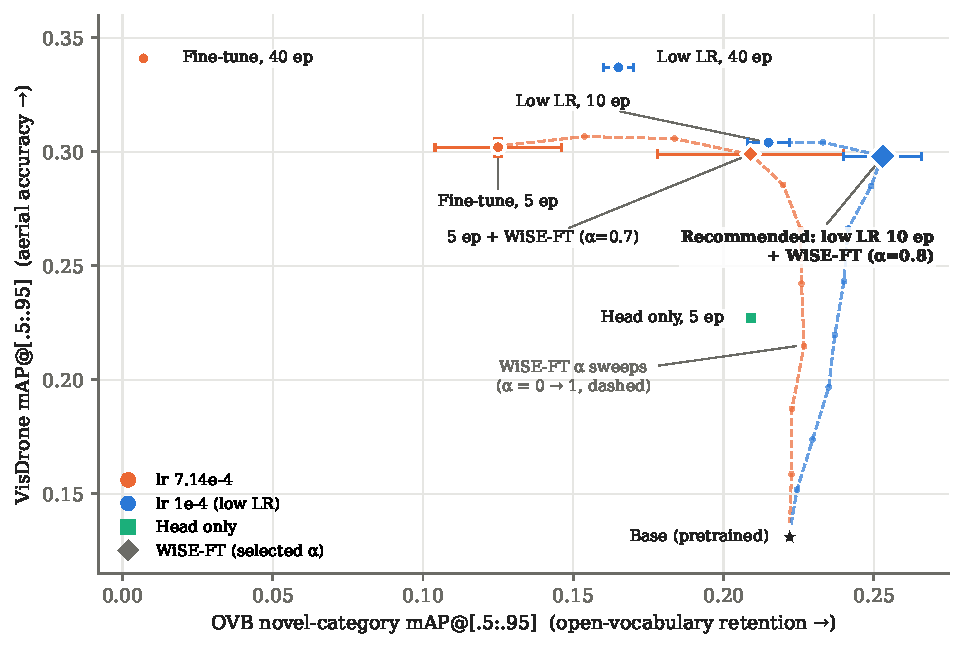
\includegraphics[width=0.8\textwidth]{pareto_novel_paper.pdf}
\caption{VisDrone mAP versus novel-category OVB mAP. Points correspond to the rows of
         Table~\ref{tab:methods} (error bars: standard deviation over three seeds); dashed
         lines trace WiSE-FT interpolation from the pretrained model ($\alpha=0$) to each
         fine-tuned model ($\alpha=1$), averaged over three seeds. A lower learning rate
         combined with WiSE-FT reaches the upper right.}
\label{fig:pareto}
\end{figure}

\subsection{Descriptive Prompts and the Landing Decision}

Table~\ref{tab:perclassovb} breaks OVB down by category. Concrete object prompts recover or
improve under the recommended recipe (backpack 0.076 to 0.174, landing pad 0.398 to 0.577),
but the descriptive prompt ``foreign object on orange circle landing pad'' is the most fragile
category, falling from 0.477 to 0.261. The prompt ``foreign object on driveway'' is near zero
for every model, including the base model.

To test whether descriptive prompts catch objects that are not explicitly prompted, we
removed the backpack, dog, and soccer ball prompts and measured how many of those 200 objects
were found by a ``foreign object'' detection at confidence 0.1. Such detections rarely
localize the object itself (at most 11\% at IoU $\geq$ 0.5 for any model); instead, they flag the
obstructed pad region. 84\% of backpacks, which lie on the pad, are covered by a base-model
``foreign object on orange circle landing pad'' detection, whereas dogs and soccer balls
elsewhere in the scene are missed. Descriptive prompts therefore act as a region-level
obstruction signal, and specific prompts remain necessary for localization; the recommended
model has the highest specific-prompt recall (59\% vs.\ 53\% for the base model).

Because the landing decision is ultimately binary, we also evaluate an image-level task:
distinguishing the 91 OVB images with an obstructed pad from the 101 with a clear pad
(Table~\ref{tab:obstruction}). Scored by the descriptive prompt alone, the base model
discriminates best (AUROC 0.835) and every fine-tuned model is worse, mirroring the per-class
results. When object prompts detected inside the landing pad are also counted, the
recommended model matches the base model (AUROC 0.861 vs.\ 0.866) at the same miss rate and
with 3\% instead of 11\% false alarms at confidence 0.25, while the 5-epoch model reaches only
0.696. This combined score was defined after observing the descriptive-only results and should
be read as exploratory.

\begin{table}[hbt!]
\caption{Per-category OVB AP@[.5:.95]. FO = foreign object. Car (one ground-truth box) is omitted.}
\label{tab:perclassovb}
\centering
\begin{tabular}{lccccccc}
\hline
\textbf{Model} & \textbf{backpack} & \textbf{dog} & \textbf{ball} & \textbf{pad} & \textbf{FO on pad} & \textbf{FO on driveway} & \textbf{pedestrian} \\
\hline
Base             & 0.076 & 0.360 & 0.016 & 0.398 & 0.477 & 0.005 & 0.275 \\
Fine-tune, 5 ep  & 0.014 & 0.011 & 0.013 & 0.424 & 0.310 & 0.001 & 0.347 \\
Fine-tune, 40 ep & 0.000 & 0.000 & 0.000 & 0.042 & 0.000 & 0.000 & 0.216 \\
5 ep + WiSE-FT   & 0.050 & 0.178 & 0.025 & 0.547 & 0.451 & 0.001 & 0.379 \\
Recommended      & 0.174 & 0.423 & 0.017 & 0.577 & 0.261 & 0.026 & 0.377 \\
\hline
\end{tabular}
\end{table}

\begin{table}[hbt!]
\caption{Image-level landing-pad obstruction detection on OVB (91 obstructed, 101 clear).
         AUROC with 95\% bootstrap CI. Descriptive: maximum confidence of the ``foreign object
         on orange circle landing pad'' prompt. Combined: additionally counts object prompts
         detected inside the landing pad. Miss and false-alarm rates for the combined score at
         confidence 0.25.}
\label{tab:obstruction}
\centering
\begin{tabular}{lcccc}
\hline
\textbf{Model} & \textbf{AUROC (descriptive)} & \textbf{AUROC (combined)} & \textbf{Miss} & \textbf{False alarm} \\
\hline
Base             & 0.835 [0.774, 0.893] & 0.866 [0.813, 0.920] & 0.54 & 0.11 \\
Fine-tune, 5 ep  & 0.668 [0.590, 0.746] & 0.696 [0.620, 0.773] & 0.81 & 0.02 \\
Fine-tune, 40 ep & 0.421 [0.354, 0.491] & 0.421 [0.354, 0.491] & 1.00 & 0.00 \\
5 ep + WiSE-FT   & 0.759 [0.687, 0.826] & 0.818 [0.755, 0.874] & 0.76 & 0.01 \\
Recommended      & 0.682 [0.602, 0.756] & 0.861 [0.806, 0.908] & 0.54 & 0.03 \\
\hline
\end{tabular}
\end{table}

\subsection{Embedded Deployment}

The 5-epoch fine-tuned checkpoint was first evaluated for real-time inference on the Jetson
Xavier and the Jetson Orin Nano using the PyTorch runtime at 1280$\times$1280, reaching 9.4 and
12.5 FPS respectively. Embedded inference on {NVIDIA} Jetson platforms has been demonstrated
across a range of real-time computer vision tasks, with the Jetson ecosystem providing a
practical deployment target for {UAS} onboard computing~\cite{mittal2019survey}. We further
benchmarked the models on an NVIDIA Jetson AGX Thor (120~W mode) with PyTorch and TensorRT,
measuring end-to-end latency (preprocessing, inference, and non-maximum suppression) at batch
size 1 over 300--500 frames held in memory, and re-scoring accuracy with each runtime
(Table~\ref{tab:thor}). TensorRT FP16 runs at 56--57 FPS with accuracy identical to PyTorch.
INT8 quantization adds only 2--4\% throughput, because CPU-side preprocessing and
non-maximum suppression dominate the frame time, and it reduces accuracy slightly, so FP16 is
the preferred configuration. The TensorRT engine embeds the prompt vocabulary and must be
rebuilt when the prompt list changes (about 2.5 minutes for FP16).

\begin{table}[hbt!]
\caption{Real-time inference at 1280$\times$1280. Xavier and Orin Nano: 5-epoch model,
         PyTorch. Thor: end-to-end latency, batch 1, 120~W mode.}
\label{tab:thor}
\centering
\begin{tabular}{llcccc}
\hline
\textbf{Platform / model} & \textbf{Runtime} & \textbf{FPS} & \textbf{p99 latency (ms)} & \textbf{VisDrone mAP} & \textbf{OVB novel} \\
\hline
Xavier, 5 ep        & PyTorch        & 9.4  & -- & -- & -- \\
Orin Nano, 5 ep     & PyTorch        & 12.5 & -- & -- & -- \\
Thor, 5 ep          & PyTorch FP32   & 35 & 32.1 & 0.308 & 0.126 \\
Thor, 5 ep          & TensorRT FP16  & 57 & 22.1 & 0.308 & 0.128 \\
Thor, 5 ep          & TensorRT INT8  & 59 & 20.8 & 0.300 & 0.119 \\
Thor, recommended   & TensorRT FP16  & 56 & 22.0 & 0.297 & 0.247 \\
\hline
\end{tabular}
\end{table}

All three platforms sustain real-time inference at full resolution, confirming that the
fine-tuned open-vocabulary detector is practical for onboard UAS deployment.

\begin{figure}[hbt!]
\centering
\begin{subfigure}{0.45\textwidth}
    \centering
    \includegraphics[height=4cm, keepaspectratio]{baseline_4.png}
    \caption{Base YOLOv8m-WorldV2 model.}
    \label{fig:pedestrian_base}
\end{subfigure}
\hfill
\begin{subfigure}{0.45\textwidth}
    \centering
    \includegraphics[height=4cm, keepaspectratio]{finetuned_4.png}
    \caption{Fine-tuned (5 epoch).}
    \label{fig:pedestrian_ft}
\end{subfigure}
\caption{Base model (left) vs.\ 5-epoch fine-tuned model (right)
         on top-down pedestrian detection.}
\label{fig:pedestrian_comparison}
\end{figure}

\begin{figure}[hbt!]
\centering
\begin{subfigure}{0.45\textwidth}
    \centering
    \includegraphics[height=4cm, keepaspectratio]{landing_pad_backpack_before_ov_loss.png}
    \caption{Base YOLOv8m-WorldV2 model.}
    \label{fig:backpack_base}
\end{subfigure}
\hfill
\begin{subfigure}{0.45\textwidth}
    \centering
    \includegraphics[height=4cm, keepaspectratio]{landing_pad_backpack_after_ov_loss.png}
    \caption{Fine-tuned (5 epoch).}
    \label{fig:backpack_ft}
\end{subfigure}
\caption{Base model (left) vs.\ 5-epoch fine-tuned model (right).
         Even short fine-tuning durations reduce detection confidence
         on open-vocabulary classes outside the VisDrone distribution.}
\label{fig:backpack_comparison}
\end{figure}

\section{Discussion}

The results reveal a clear tradeoff between domain specialization and open-vocabulary
retention, but one that depends far more on how the model is fine-tuned than on how long.
Even with the CLIP text encoder frozen, updating the visual backbone, neck, and detection head
at a learning rate of $7.14\times10^{-4}$ degrades detection of unseen categories within a few
hundred iterations and removes it almost entirely by 40 epochs. Fig.~\ref{fig:backpack_comparison}
illustrates this: detection confidence on the prompted OVB class ``backpack'' decreases after
fine-tuning, while Fig.~\ref{fig:pedestrian_comparison} shows the dramatic improvement on
VisDrone classes such as ``pedestrian.'' Freezing the text encoder is therefore necessary but
not sufficient. Our results point to the size of the update in weight space as the governing
factor: a lower learning rate keeps the visual components close to the pretrained solution
over long training, and interpolating back toward the pretrained weights recovers most of what
is lost. Layer freezing, by contrast, restricts which weights move but not how far, and only
delays the collapse.

The benchmark used to measure retention matters. OVB retention overstated general retention:
the 5-epoch model kept 58\% of base novel OVB mAP but only 18--19\% of base LVIS and COCO AP. The
recommended model retains 77--78\% on LVIS and COCO and slightly exceeds the base model on
novel OVB categories, so the gain is not specific to our benchmark. Descriptive noun phrases
are the most fragile capability. Concrete object prompts recover under the recommended recipe,
but ``foreign object on orange circle landing pad'' does not, and ``foreign object on
driveway'' fails for every model. In practice the descriptive prompt behaves as a region-level
signal that the pad is occupied rather than as a detector of arbitrary objects, and it is most
useful when combined with an exhaustive list of specific hazard prompts. Under that
combination the recommended model matches the base model at deciding whether the pad is
obstructed while raising far fewer false alarms.

Several limitations bound these findings. The 195-image OVB set is small and comes from a
single site; we mitigate this with bootstrap confidence intervals, three-seed repetitions,
novel-only reporting, and standard benchmarks, but absolute OVB values should be interpreted
with caution. Standard-benchmark and learning-rate-grid results are single-seed. The
image-level obstruction labels are derived from the OVB annotations, and the combined
obstruction score was defined after inspecting the results; at confidence 0.25 all models
miss more than half of obstructed pads, so an operational system would require a lower,
calibrated threshold validated on substantially more data. We did not compare against
closed-set detectors trained on the same data.

A practical limitation of this approach is that target classes must be prompted before
inference, requiring prior knowledge of potential obstructions. This can be partially
addressed using an exhaustive prompt list of common hazard categories combined with
descriptive prompts for the landing pad region. Future work will explore using
vision-language models, either cloud-based or compact onboard models such as
LiteVLM~\cite{huang2025litevlmlowlatencyvisionlanguagemodel}, to dynamically generate prompts
from a scene prior to YOLO-World inference, as well as parameter-efficient fine-tuning and
replay of pretraining data as further retention strategies.

\section{Conclusion}

This paper presented a fine-tuning methodology for adapting YOLO-World to UAS landing zone
obstruction detection and characterized the tradeoff between VisDrone accuracy and
open-vocabulary retention. Freezing the CLIP text encoder alone is not sufficient: standard
fine-tuning significantly degrades detection of unseen categories within 5 epochs and
eliminates it by 40. The learning rate, more than training duration or layer freezing,
primarily governs this loss. A low learning rate combined with weight-space ensembling yields
a model that more than doubles VisDrone accuracy (+137\% mAP@0.5) while retaining 77--78\% of
the pretrained model's zero-shot accuracy on LVIS and COCO and slightly exceeding it on novel
UAS obstruction categories. Combined with specific hazard prompts, its descriptive landing-pad
prompt identifies obstructed landing pads as well as the pretrained model with a
3.6$\times$ lower false-alarm rate, and TensorRT deployment reaches 56 FPS at full resolution
on an NVIDIA Jetson AGX Thor. These results establish a practical foundation for
open-vocabulary obstruction detection in autonomous UAS landing and motivate future work on
dynamic prompt generation via vision-language model integration.

% \section*{Acknowledgments}

% ...

\bibliography{sample}
% \bibliographystyle{aiaa}  % new-aiaa.cls already sets new-aiaa; a second style makes BibTeX error

\end{document}
